\documentclass{article}
\usepackage{graphicx}
\usepackage[french]{babel}
\usepackage{fullpage}
\advance\hoffset by -3mm  % A4 is narrower.
\advance\voffset by  8mm  % A4 is taller.
\newtheorem{definition}{D\'efinition}
\title{Pratique du~C (INFO~$301$)~:\\
  Projet~: implantation du filtre grep} \begin{document}
\maketitle
\section{Introduction}
On se propose d'implanter en C-ANSI un filtre \texttt{mongrep} inspir\'e du
filtre \texttt{grep} existant sur la plupart des syst\`emes Unix.
\par
Bien que certaines notions utilis\'ees dans ce projet vous sont
famili\`eres puisque vues en cours de compilation, le sujet est
autosuffisant et ne n\'ecessite pas la ma\^\i{}trise de ce cours.
\par
Le filtre \texttt{mongrep} imprime les lignes, appartenant \`a un
fichier, qui contiennent un certain \emph{motif}. Ce dernier
correspond \`a l'ensemble des mots d'un \emph{langage} reconnu par un
automate associ\'e \`a une \emph{expression rationnelle}.  
\par
Le motif recherch\'e est donn\'e par l'utilisateur
dans la ligne de commande sous la forme d'un param\`etre
repr\'esentant une expression rationnelle (cf.\ section~\ref{ser:details} page~\pageref{ser:details}).
\par
 Le filtre \texttt{mongrep}
doit donc reconna\^\i{}tre le langage associ\'e pour effectuer la
recherche du motif.
\par
Pour toute expression rationnelle, il existe un unique (au nom des
\'etats pr\`es) automate fini d\'eterministe minimal
\emph{reconnaissant} le langage associ\'e. La construction d'un tel
automate passe par
\begin{enumerate}
\item la construction d'un arbre de syntaxe abstraite associ\'e \`a
  l'expression rationnelle~; 
\item la construction d'un automate fini %d\'eterministe
 \`a partir de  cet arbre~;
%\item la minimisation de cet automate d\'eterministe.
\end{enumerate}
Nous allons coder ces phases qui nous seront suffisantes (sans aller jusqu'\`a construire un automate fini d\'eterministe). % bien que la derni\`ere ne soit pas
%imp\'erative \`a l'implantation du filtre~\texttt{mongrep}.
\section{Une grammaire d'expressions rationnelles}
\label{sec:GramExpRat}
La grammaire des expressions rationnelles utilis\'ees par la
commande~\texttt{mongrep} est donn\'ee par la Figure~\ref{grammaire}
page~\pageref{grammaire}. C'est une version tr\`es simplifi\'ee de
celle utilis\'ee par \texttt{grep}.
\begin{figure}
{\normalsize
\begin{verbatim}
expression ::= expression_concatenation '|' expression || expression_concatenation
expression_concatenation ::= expression_repetition expression_concatenation 
                             || expression_repetition
expression_repetition ::= expression_simple '*' || expression_simple
expression_simple ::= '(' expression ')' || car_non_speciaux || intervalle
car_non_speciaux ::= tout caractere sauf '|', '*', '[', ']', '.' || '\|' || '\*' 
                     || '\[' || '\]' || '\.'
intervalle ::= '.' || '[' liste ']' || '[^' liste ']' || '[' liste '-]' 
               || '[^' liste '-]'
liste ::= non_moins liste1 
liste1 ::= non_fermant liste1
non_moins ::= tout caractere sauf '-'
non_fermant ::= tout caractere sauf ']'
\end{verbatim}
}
\caption{Grammaire des expressions rationnelles de \texttt{mongrep}
  \label{grammaire}}
\end{figure}
Notre filtre \texttt{mongrep} va prendre une cha\^\i{}ne de
caract\`eres codant une expression rationnelle en param\`etre depuis
la ligne de commande d'un shell. Dans un premier temps, cette
cha\^\i{}ne va \^etre convertie en un arbre binaire d\'enomm\'e
\emph{arbre de syntaxe abstraite}.
%% -------------------------------------------------------------------------
\section{Construction d'un arbre de syntaxe abstraite correspondant
  \`a une expression rationnelle}
La Figure~\ref{arbre} page~\pageref{arbre} sch\'ematise la repr\'esentation d'un tel arbre
et les principales fonctions permettant sa construction \`a partir
d'une cha\^\i{}ne de caract\`eres --- prise sur l'entr\'ee standard
--- pour une grammaire simplifi\'ee.
\begin{figure}
  \begin{center}
    \leavevmode
    \includegraphics[width=\textwidth]{asa}
  \end{center}
  \caption{Construction de l'arbre \label{arbre}}
\end{figure}
Pour \^etre plus pr\'ecis, la fonction \texttt{simple} de la Figure~\ref{arbre}  page~\pageref{arbre}  
implante la r\`egle
\begin{verbatim}
simple ::= '(' expr ')' || car 
\end{verbatim}
de la grammaire simplifi\'ee.
\par
Notez bien qu'en ce qui concerne le filtre \texttt{mongrep} que l'on
vous demande d'implanter, la cha\^\i{}ne de caract\`eres
repr\'esentant l'expression rationnelle consid\'er\'ee n'est pas prise
sur l'entr\'ee standard --- comme dans l'exemple de la Figure~\ref{arbre} ---
mais comme param\`etre du filtre. 
Ainsi, on vous demande d'adapter le code de
la Figure~\ref{arbre} page~\pageref{arbre} afin d'\^etre utilisable
dans le filtre \texttt{mongrep} et de le compl\'eter afin de pouvoir
implanter la grammaire de la Figure~\ref{grammaire}
page~\pageref{grammaire}.
\par
Les algorithmes pr\'esent\'es dans la suite utilisent l'arbre de
syntaxe abstraite construit pr\'ec\'edemment, auquel on a ajout\'e un
n\oe{}ud racine (de type~\verb+CONCAT+) ayant pour fils droit un
n\oe{}ud de fin~$\textrm{end}$ (not\'e \# dans la Figure~\ref{arbre})
et pour fils gauche l'arbre de syntaxe abstrait originel.
%% -------------------------------------------------------------------------
% \documentclass{article}

% \usepackage[utf8]{inputenc} 
% \usepackage[french]{babel} 
% \usepackage{portland} 
% \usepackage{epsfig} 
% \usepackage{url} 
% \usepackage{hyperref} 
% \usepackage{fancybox} 
% \usepackage{pgf}

% \pgfdeclareimage[height=12cm]{arbre}{arbre}
% \pgfdeclareimage[width=\textwidth]{automate}{automate}

% %\newtheorem{exemple}{Exemple} 
% \newtheorem{definition}{D{\'e}finition} 
% %\newtheorem{remarque}{Remarque} 
% %\newtheorem{question}{Question} 
% %\newtheorem{notation}{Notation} 
% %\newtheorem{remarques}{Remarques} 

% \title{Grep : construire l'automate}

% \begin{document}
% \maketitle


\section{Construction d'un automate non d{\'e}terministe {\`a} partir d'un arbre de syntaxe abstraite}

Illustrons la m{\'e}thode {\`a} l'aide d'un exemple. Consid\'erons l'expression rationnelle~: 
\[ (ab+c)^\star ab \] correspondant {\`a} l'arbre de syntaxe de la Figure~\ref{as} page~\pageref{as}. 
Le but de l'algorithme est de construire l'automate de la Figure~\ref{au} page~\pageref{au}.
\begin{figure}
\begin{center}
  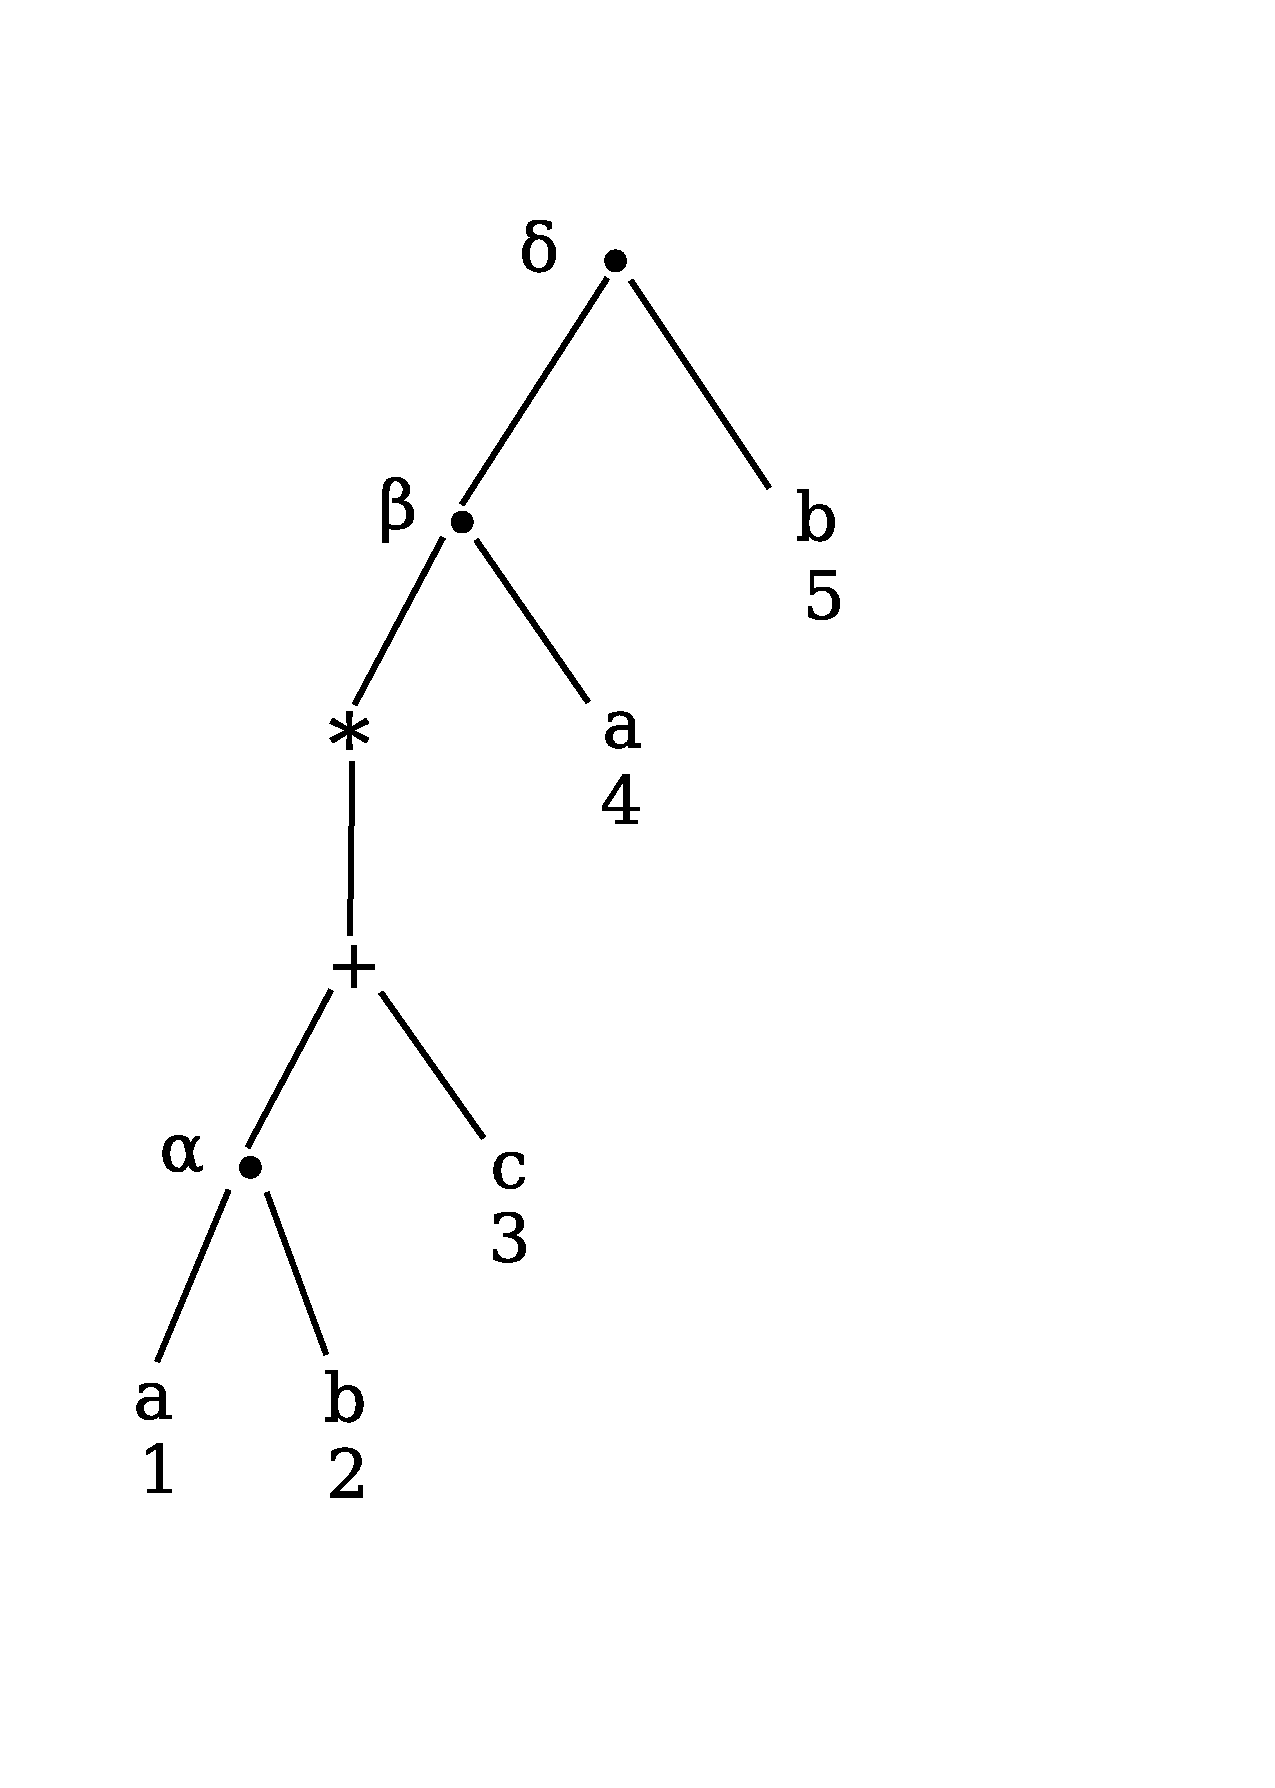
\includegraphics[width=5cm]{arbre}
%\pgfuseimage{arbre}
\caption{\label{as} Arbre syntaxique de l'expression rationnelle $(ab+c)^\star ab$}
\end{center}
\end{figure}
\begin{figure}
\begin{center}
\includegraphics[width=10cm]{automate}
%\pgfuseimage{automate}
\caption{\label{au} automate non d{\'e}terministe construit {\`a} partir de l'expression rationnelle $(ab+c)^\star ab$}
\end{center}
\end{figure}
Commen\c{c}ons par introduire un peu de terminologie.
\begin{definition}
Etant donn{\'e}e une expression rationnelle, on d{\'e}finit une \emph{position} dans cette expression comme l'indice d'un des 
caract{\`e}res alphab{\'e}tiques la composant. 
Pour l'expression $(ab+c)^\star ab$, il y a cinq positions : 
\[ 1) \, a,  \quad 2) \, b, \quad 3) \, c, \quad 4) \, a, \quad 5)\, b.\]
\end{definition}

L'automate de la Figure~\ref{au} page~\pageref{au}  a les caract{\'e}ristiques suivantes~: 
\begin{itemize}
\item un {\'e}tat initial $O$~;
\item un {\'e}tat par positions (i.e.\ caract{\`e}re alphab{\'e}tique de l'expression
  rationnelle)~;
\item depuis l'{\'e}tat initial, on peut se rendre sur les {\'e}tats
  correspondant aux positions o{\`u} peut commencer un mot
  v{\'e}rifiant l'expression rationnelle ($1, 3$ ou~$4$)~;
\item les {\'e}tats terminaux correspondent aux positions o{\`u} cette
  expression peut se terminer. En l'occurence, l'expression
  consid{\'e}r{\'e}e ne peut se terminer qu'apr{\`e}s le 'b' final
  (position 5).
\end{itemize}
\paragraph{Interpr\'etation de l'automate.}
Informellement, l'automate permet de coder l'information suivante~: 
\begin{quote}
\'etant  dans l'{\'e}tat~$i$, quelle peut {\^e}tre la lettre suivante, et en quelle position m'am{\`e}nera-t-elle~? 
\end{quote}
Par exemple, depuis l'{\'e}tat~$2$ (dans la lecture de l'expression rationnelle, on vient de lire le premier b) : 
\begin{itemize}
\item on peut lire un c (application de l'{\'e}toile, choix de c) et arriver en position~$3$~;
\item on peut lire un a (application de l'{\'e}toile, choix de ab) et revenir en position~$1$~; 
\item on peut lire un a (sortie de l'{\'e}toile, lecture du caract{\`e}re suivant) et arriver en position~$4$. 
\end{itemize}
Chacune de ces options correspond {\`a} une transition dans l'automate, qui repr{\'e}sente ainsi toutes les transitions possibles engendr{\'e}es par ce raisonnement.
\paragraph{Indicateurs.}
Avant d'automatiser le processus, et trouver un algorithme permettant de construire l'automate {\`a} partir
de l'expression rationnelle, on peut d{\'e}gager trois notions importantes~: 
\begin{itemize}
\item par quels caract{\`e}res peut commencer un mot v{\'e}rifiant une expression rationnelle donn{\'e}e~? (ou dit autrement, par quelle position peut-on 'entrer' dans une expression rationnelle~?)
\item par quels caract{\`e}res (quelles positions) peut se terminer un mot v{\'e}rifiant une expression rationnelle~? 
(par quelle position peut-on 'sortir' d'une expression rationnelle~?)
\item \`a partir d'une position donn{\'e}e, quelles sont les positions accessibles~? 
\end{itemize}
Il existe une derni{\`e}re notion {\`a} envisager, qui n'est pas illustr\'ee par notre exemple~: 
\begin{itemize}
\item \`a partir d'une position, peut-on reconna{\^\i}tre le mot vide~$\epsilon$~? 
\end{itemize}
\begin{definition}
Ces quatre notions (indicateurs) seront nomm{\'e}es dans l'ordre~: 
\begin{itemize}
\item $\mbox{first}(i)$~: ensemble des positions par lesquelles peut commencer une expression rationnelle~;
\item $\mbox{last}(i)$~: ensemble des positions o{\`u} peut se terminer une expression rationnelle~;
\item $\mbox{follow}(i)$~: ensemble des positions accessibles depuis la position~$i$~;
\item $\mbox{nullable}(i)$~: vrai si $\epsilon$ est reconnu depuis cette position. 
\end{itemize}
\end{definition}
L'arbre de syntaxe d{\'e}coupe l'expression rationnelle en sous-expressions. Les quatre indicateurs peuvent donc {\^e}tre d{\'e}finis en chaque n\oe ud de l'arbre, puisque chacun de ces n\oe{}uds est lui-m{\^e}me la racine d'une expression rationnelle.

\subsection{Indicateurs pour les feuilles}
Les feuilles sont de trois types~$\emptyset, \epsilon$ ou~$i$~; les valeurs des indicateurs pour chaque type de feuille se d{\'e}finissent facilement~: 
\begin{itemize}
\item N\oe{}ud $\emptyset$ : $\mbox{nullable}=\mbox{false}$, $\mbox{first}=\mbox{last}=\mbox{follow}=\emptyset$~;
\item N\oe{}ud $\epsilon$ : $\mbox{nullable}=\mbox{true}$, $\mbox{first}=\mbox{last}=\mbox{follow}=\emptyset$~;
\item N\oe{}ud position $i$ : $\mbox{nullable}=\mbox{false}$, $\mbox{first}(i)=\mbox{last}(i)=\{i\}$, $\mbox{follow}(i)=\emptyset$.
\end{itemize}
\subsection{Indicateurs pour les n\oe{}uds internes}
Il y a trois types de n\oe{}uds internes : concat{\'e}nation, {\'e}toile, union. Pour chacun de ces types de n\oe{}ud, on peut calculer les indicateurs correspondants, {\`a} partir des indicateurs de leur(s) descendant(s). 

\subsubsection{N\oe{}ud concat\'enation}
Dans cette section, nous allons consid\'erer comment d\'eterminer les indicateurs d'un n\oe{}ud concat\'enation.
\paragraph{nullable.}
Un n\oe{}ud concat{\'e}nation peut engendrer $\epsilon$ si son fils gauche (g) et son fils droit (d) sont capables d'engendrer $\epsilon$ :

$$\mbox{nullable}(g \bullet d)=\mbox{nullable}(g) \mbox{ et } \mbox{nullable}(d).$$
\paragraph{first.}
Pour un n\oe{}ud concat{\'e}nation, les positions pouvant commencer un mot sont~:
\begin{itemize}
\item  celles pouvant commencer son fils gauche~;
\item et seulement si son fils gauche peut engendrer $\epsilon$, les positions pouvant d{\'e}buter un mot du fils droit.
\end{itemize}

$$
\mbox{first}(g\bullet d)=\left\{
\begin{array}{l}
\mbox{first}(g) \mbox{ si } \mbox{nullable}(g)= \mbox{false}, \\
\mbox{first}(g)\cup \mbox{first}(d) \mbox{ si } \mbox{nullable}(g)=\mbox{true}.
\end{array}
\right.
$$
\paragraph{last.}
Les positions susceptibles de terminer un mot d'un n\oe{}ud concat{\'e}nation sont~:
\begin{itemize}
\item  celles qui peuvent terminer son fils droit~;
$$\mbox{last}(g\bullet d)=\mbox{last}(d) \mbox{ si } \mbox{nullable}(d)= \mbox{false},$$
\item auxquelles on ajoute celles terminant son fils gauche, si le fils droit peut engendrer $\epsilon$~:
$$\mbox{last}(g\bullet d)=\mbox{last}(g)\cup \mbox{last}(d) \mbox{ si } \mbox{nullable}(d)=\mbox{true}.$$
\end{itemize}
Donc, on a~:
$$\mbox{last}(g\bullet d)=\left\{
\begin{array}{l}
\mbox{last}(d) \mbox{ si } \mbox{nullable}(d)= \mbox{false},\\
\mbox{last}(g)\cup \mbox{last}(d) \mbox{ si } \mbox{nullable}(d)=\mbox{true}.
\end{array}
\right.
$$
\paragraph{follow.}
Soit $x$ une position dans $g\bullet d$. 
\begin{itemize}
\item Si $x$ est dans $d$, les positions qui peuvent lui succ{\'e}der sont les m{\^e}mes que celles qui peuvent lui succ\'eder dans $d$ : 

$$\mbox{follow}(g\bullet d,x)=\mbox{follow}(d,x)~;$$

\item Si $x$ est dans $g$, mais n'appartient pas {\`a} $\mbox{last}(g)$, les positions qui peuvent lui succ{\'e}der sont les m{\^e}mes que celles qui peuvent lui succ\'eder dans $g$ : 

$$\mbox{follow}(g\bullet d,x)=\mbox{follow}(g,x)~;$$

\item Si $x$ est dans~$\mbox{last}(g)$, les positions suivant $x$ sont celles lui succ{\'e}dant dans $g$, auxquelles on ajoute toutes les positions pouvant commencer $d$ : 

$$\mbox{follow}(g\bullet d,x)=\mbox{follow}(g,x) \cup \mbox{first}(d).$$

\end{itemize}

\subsubsection{N\oe{}ud union}
\paragraph{nullable.}
Un n\oe{}ud union ($g+d$) permet d'engendrer $\epsilon$ si l'un de ses fils au moins peut le faire~: 
$$\mbox{nullable}(g + d)=\mbox{nullable}(g)\ \mbox{or}\ \mbox{nullable}(d).$$
\paragraph{first.}
Les positions pouvant commencer un mot d{\'e}fini par un n\oe{}ud union sont celles permettant de commencer un mot de $g$ plus celles pouvant comencer un mot de $d$~: 
$$\mbox{first}(g + d)=\mbox{first}(g) \cup \mbox{first}(d).$$ 
\paragraph{last.}
M{\^e}me raisonnement pour les fins de mots~: 
$$\mbox{last}(g + d)=\mbox{last}(g) \cup \mbox{last}(d).$$ 
\paragraph{follow.}
Si $x$ est une position de $g + d$, elle est soit une position de $g$, soit une position de $d$. On a donc simplement : 
$$\mbox{follow}(g +d,x)=\left\{
\begin{array}{ll}
\mbox{follow}(g,x)&  \mbox{ si }x \in g,\\
\mbox{follow}(d,x)& \mbox{ si } x \in d.
\end{array}
\right.$$
\subsubsection{N\oe{}ud {\'e}toile}
\paragraph{nullable.}
Une expression {\`a} l'{\'e}toile peut engendrer epsilon : 

$$\mbox{nullable}(\star)=\mbox{true}.$$
\paragraph{first et last. }
Les positions pouvant commencer un mot correspondant {\`a} une expression {\`a} l'{\'e}toile sont exactement celles qui permettent de commencer un mot du langage de base. Idem pour les positions en fin d'expression : 
$$\mbox{first}(g^\star)=\mbox{first}(g),\quad\quad \mbox{last}(g^\star)=\mbox{last}(g).$$
\paragraph{follow.}
Si $x \not\in \mbox{last}(g)$, alors les positions qui peuvent lui succ{\'e}der sont celles qui pouvaient lui succ{\'e}der dans $g$.
Sinon, il faut y ajouter les d{\'e}buts possibles de mots de $g$, qui viendront se concat{\'e}ner derri{\`e}re $x$ : 
$$\mbox{follow}(g^\star,x)=\left\{
\begin{array}{ll}
\mbox{follow}(g,x)& \mbox{ si } x \not\in \mbox{last}(g), \\
\mbox{follow}(g,x)\cup \mbox{first}(g)& \mbox{ si } x \in \mbox{last}(g).
\end{array}
\right.
$$
\subsection{Exemple d'application}

On reprend l'arbre de syntaxe de la Figure~\ref{as} page~\pageref{as}, o{\`u} figurent les num{\'e}ros des positions. 
Nous partons des feuilles pour remonter {\`a} la racine. Lorsque vous le programmerez, une approche r{\'e}cursive sera plus facile {\`a} concevoir. 

Pour la position 1 : 

$$\begin{array}{lcl}
\mbox{nullable}(1)&=&\mbox{false},\\
\mbox{first}(1)&=&\{1\},\\
\mbox{last}(1)&=&\{1\},\\
\mbox{follow}(1)&=&\emptyset.
\end{array}
$$

Pour la position 2 : 

$$\begin{array}{lcl}
\mbox{nullable}(2)&=&\mbox{false},\\
\mbox{first}(2)&=&\{2\},\\
\mbox{last}(2)&=&\{2\},\\
\mbox{follow}(2)&=&\emptyset.
\end{array}
$$

Pour le n\oe{}ud interne $1\bullet \alpha2$ : 
$$\begin{array}{lcl}
\mbox{nullable}&=&\mbox{false},\\
\mbox{first}&=&\{1\},\\
\mbox{last}&=&\{2\},\\
\mbox{follow}(1)&=&\{2\},\\
\mbox{follow}(2)&=&\emptyset.
\end{array}
$$

Pour la position 3 : 

$$\begin{array}{lcl}
\mbox{nullable}(3)&=&\mbox{false},\\
\mbox{first}(3)&=&\{3\},\\
\mbox{last}(3)&=&\{3\},\\
\mbox{follow}(3)&=&\emptyset.
\end{array}
$$

Pour le n\oe{}ud $+$ : 
$$\begin{array}{lcl}
\mbox{nullable}&=&\mbox{false},\\
\mbox{first}&=&\{1,3\},\\
\mbox{last}&=&\{2,3\},\\
\mbox{follow}(1)&=&\{2\},\\
\mbox{follow}(2)&=&\emptyset,\\
\mbox{follow}(3)&=&\emptyset.
\end{array}
$$

Pour le n\oe{}ud interne $1\star2$ : 
$$\begin{array}{lcl}
\mbox{nullable}&=&\mbox{true},\\
\mbox{first}&=&\{1,3\},\\
\mbox{last}&=&\{2,3\},\\
\mbox{follow}(1)&=&\{2\},\\
\mbox{follow}(2)&=&\{1,3\},\\
\mbox{follow}(3)&=&\{1,3\}.
\end{array}
$$

Pour la position 4~: 

$$\begin{array}{lcl}
\mbox{nullable}(4)&=&\mbox{false},\\
\mbox{first}(4)&=&\{4\},\\
\mbox{last}(4)&=&\{4\},\\
\mbox{follow}(4)&=&\emptyset.
\end{array}
$$

Pour le n\oe{}ud interne $1\bullet \beta2$ : 
$$\begin{array}{lcl}
\mbox{nullable}&=&\mbox{false},\\
\mbox{first}&=&\{1,3,4\},\\
\mbox{last}&=&\{4\},\\
\mbox{follow}(1)&=&\{2\},\\
\mbox{follow}(2)&=&\{1,3,4\},\\
\mbox{follow}(3)&=&\{1,3,4\},\\
\mbox{follow}(4)&=&\emptyset.
\end{array}
$$

Pour la position 5~: 

$$\begin{array}{lcl}
\mbox{nullable}(5)&=&\mbox{false},\\
\mbox{first}(5)&=&\{5\},\\
\mbox{last}(5)&=&\{5\},\\
\mbox{follow}(5)&=&\emptyset.
\end{array}
$$


enfin, au sommet de l'arbre, pour la position $\bullet \delta$

$$\begin{array}{lcl}
\mbox{nullable}&=&\mbox{false},\\
\mbox{first}&=&\{1,3,4\},\\
\mbox{last}&=&\{5\},\\
\mbox{follow}(1)&=&\{2\},\\
\mbox{follow}(2)&=&\{1,3,4\},\\
\mbox{follow}(3)&=&\{1,3,4\},\\
\mbox{follow}(4)&=&\{5\},\\
\mbox{follow}(5)&=&\emptyset.
\end{array}
$$


Ces derni{\`e}res informations permettent de d{\'e}finir enti{\`e}rement l'automate : 
\begin{itemize}
\item l'{\'e}tat initial n'est pas final (le n\oe{}ud au sommet de l'arbre n'est pas $\mbox{nullable}$)~;
\item $\mbox{follow}$ fournit la table de transition de l'automate, aid{\'e} par $\mbox{first}$ qui d{\'e}crit les transitions depuis l'{\'e}tat initial~;
\item $\mbox{last}$ donne la liste, ici r{\'e}duite {\`a} un seul {\'e}tat, des {\'e}tats terminaux. 
\end{itemize}
\par\medskip

Il vous reste encore {\`a} d{\'e}finir une structure de donn{\'e}es pour l'automate, ainsi que les fonctions permettant de s'y d{\'e}placer. 
\paragraph{Attention.} L'automate est non d{\'e}terministe~; vous devrez g{\'e}rer une liste d'{\'e}tats accessibles~: un mot sera reconnu si un {\'e}tat final appartient {\`a} cette liste lorsque le mot aura {\'e}t{\'e} compl{\`e}tement lu. 




%% -------------------------------------------------------------------------
%  \subsection{Construction de l'automate d\'eterministe}
%  Pour obtenir l'automate d\'eterministe \`a partir de ces ensembles, il
%  reste \`a appliquer l'algorithme pr\'esent\'e Fig.~\ref{determ}
%  page~\pageref{determ}. Cet algorithme construit un ensemble
%  d'\'etats~$Detat$, chaque \'etat \'etant associ\'e \`a un sous-arbre
%  de l'arbre de syntaxe abstraite, et une table de transition~$Dtran$,
%  repr\'esentant les transitions de l'automate. Ainsi, si~${Dtran[T, a]
%    = U}$, alors il y a une transition dans l'automate de l'\'etat~$T$
%  \`a l'\'etat~$U$ \'etiquet\'ee par la lettre~$a$. \par Les \'etats
%  de~$Detat$ sont marqu\'es pour pouvoir indiquer s'ils ont \'et\'e
%  examin\'es ou pas. L'\'etat initial de l'automate
%  est~$\textrm{initial}(root)$, les \'etats finaux sont tous les \'etats
%  associ\'e au n\oe{}ud repr\'esentant le symbole de fin.
%  \begin{figure}[htbp]
%    {\bf Initialement},~$Detat$ contient un seul \'etat non marqu\'e
%    constitu\'e des \'el\'ements de~$\textrm{initial}(root)$.
%    \par
%    {\bf Tant qu'}il reste un \'etat~$T$ non marqu\'e dans~$Detat$ {\bf
%      faire}
%    \begin{itemize}
%    \item marquer~$T$;
% %        \item {\bf Pour} chaque lettre~$a$ de l'alphabet {\bf faire}
% %          \begin{itemize}
% %          \item Soit~$U$ l'ensemble des n\oe{}uds de l'arbre qui sont
% %            dans~$\textrm{follow}(p)$, avec~$p$ le n\oe{}ud
% %            associ\'e
% %            \`a~$T$, et tel que~$p$ repr\'esente la lettre~$a$~;
% %          \item {\bf Si}~$U$ n'est pas vide et n'appartient pas
% %            \`a~$Detat$, {\bf alors} ajouter~$U$ \`a~$Detat$ (sans
% %            le
% %            marquer)~;
% %          \item $Dtran[T, a] = U$~;
% %          \end{itemize}
% %        \end{itemize}
%  \item[] Soit~$U$ l'ensemble des n\oe{}uds de l'arbre qui sont
%    dans~$\textrm{follow}(p)$, avec~$p$ le n\oe{}ud associ\'e
%    \`a~$T$. \par
%    Pour tout \'el\'ement de~$u$ de~$U$ faire~: \begin{itemize} \item
%      {\bf Si} $u$ qui n'appartient pas d\'ej\`a \`a~$Detat$, {\bf
%        alors} ajouter~$u$ \`a~$Detat$ (sans le marquer)~; \item
%      ${Dtran[T, a] = u}$ pour chaque lettre~$a$ dans l'alphabet
%      associ\'e au n\oe{}ud~$p$. \end{itemize} \end{itemize}
%  \caption{Construction de l'automate d\'eterministe. \label{determ}}
%  \end{figure}
 %% -------------------------------------------------------------------------
% \subsection{Minimisation de l'automate}
% %% -------------------------------------------------------------------------
% Veuiller \`a terminer une implantation du filtre \texttt{mongrep}
% avant d'implanter cette minimisation.
% \par\medskip
% La minimisation d'un automate d\'eterministe~$M$ s'effectue en
% partitionnant l'ensemble de ses \'etats. Le calcul de cette
% partition~$\Pi_{finale}$ se fait en appliquant it\'erativement
% l'algorithme de la figure~\ref{minim} sur la partition
% courante~$\Pi$. Chaque application de cet algorithme \`a~$\Pi$
% calcule une nouvelle partition~$\Pi_{new}$, et, lorsque~${\Pi_{new}
%   = \Pi}$, on a trouv\'e la partition finale~${\Pi_{finale} =
%   \Pi_{new}}$. Si~${\Pi_{new} \neq \Pi}$, on r\'eit�re l'algorithme
% de la figure~\ref{minim} en prenant~${\Pi = \Pi_{new}}$.
% Initialement, la partition~$\Pi$ comporte deux groupes, le groupe
% des \'etats acceptants (finaux), et les \'etats non-acceptants.

% \begin{figure}[htbp] {\bf Pour} chaque groupe~$G$ de~$\Pi$ {\bf
%     faire} \begin{itemize} \item Partitionner~$G$ en sous-groupes,
%     de sorte que \begin{quote} deux \'etats~$s$ et~$t$ de~$G$ sont
%       dans le m\^eme sous-groupe {\em si et seulement si}, pour
%       toute lettre~$a$ de l'alphabet, les \'etats~$s$ et~$t$ ont une
%       transition par~$a$ vers des \'etats qui appartiennent au
%       m\^eme groupe de~$\Pi$; \end{quote} \item Remplacer~$G$
%     dans~$\Pi_{new}$ par l'ensemble des sous-groupes calcul\'es
%     pr\'ec\'edemment; \end{itemize} \caption{Algorithme de
%     partitionnement d'une partition $\Pi$.} \label{minim}
% \end{figure}

% Chaque groupe d'\'etats de~$\Pi_{finale}$ repr\'esente en fait un
% \'etat de l'automate minimal~$M'$. Pour calculer les transitions de
% l'automate minimal, on choisit pour chaque groupe de~$\Pi_{finale}$
% un \'etat {\em repr\'esentant}. Les \'etats de l'automate minimal
% seront les \'etats repr\'esentants. Soit $s$ un \'etat
% repr\'esentant, et supposons qu'il y a une transition par la lettre
% $a$ dans l'automate non minimal de $s$ vers $t$. Soit $r$ le
% repr\'esentant du groupe de $t$, alors on a une transition dans
% l'automate minimal de $s$ vers $r$ par la lettre $a$. L'\'etat
% initial de $M'$ sera le repr\'esentant du groupe contenant l'\'etat
% initial de $M$, ses \'etats finaux seront les repr\'esentants des
% groupes qui contiennent un \'etat final de $M$. Il reste \`a
% supprimer les \'etats morts (bouclant sur eux-m\^emes pour toute
% lettre) non finaux, et les \'etats non-atteignables depuis l'\'etat
% initial.

%% -------------------------------------------------------------------------
\section{Implantation de la commande \texttt{mongrep}}
%% -------------------------------------------------------------------------
\label{ser:details}
La commande \texttt{mongrep} a la syntaxe suivante:
\begin{verbatim}
mongrep  expression-rationnelle < fichier
\end{verbatim}
en utilisant la grammaire des expressions rationnelles pr\'esent\'ee
dans la section~\ref{sec:GramExpRat}. Cette commande effectue la
recherche des motifs dans le fichier envoy\'e sur son entr\'ee
standard~; elle affiche les lignes qui contiennent un mot du langage
d\'efini par l'expression rationnelle.

Remarque~: les caract\`eres ASCII constituant les m\'etacaract\`eres
sont d'abord interpr\'et\'e par le shell. Ainsi le filtre
\texttt{mongrep} doit en tenir compte comme dans les exemples
suivants --- et \'equivalents --- d'appels~:
\begin{verbatim}
% ./mongrep '(a|b)*abb' < foo # l'accent aig\"u ' bloque l\'evaluation
% ./mongrep \(a\|b\)\*abb < foo
\end{verbatim}
Le caract\`ere ASCII~\verb+\+ permet de bloquer l'\'evaluation du
m\'etacaract\`ere par le shell et permet ainsi \`a la commande
\texttt{mongrep} de le traiter. Votre filtre \texttt{mongrep} doit
permettre de consid\'erer un m\'etacaract\`ere comme un caract\`ere
ASCII normal sur le m\^eme principe (utilisation de~\verb+\+).
 
\section{R\'ealisation}
\label{sec:realisation}

Vous devez rendre (par l'interface PROF) un r\'epertoire contenant~:
\begin{itemize}
\item les codes sources de votre projet~; \item un Makefile permettant
  la compilation de votre projet~; \item un fichier de test
  \texttt{testfile} et un script shell
  \texttt{test.sh} utilisant \texttt{mongrep} sur ce fichier test.
\end{itemize} Vous pouvez adjoindre une description de votre
implantation. \end{document}
%%% Local Variables: 
%%% mode: latex
%%% TeX-master: t
%%% End: 
